\section{Smoothly Varying Costs}
The obstacle-avoiding route shown in Figure 2 is only one example among a family of possible routes of equal cost. A smoothly-varying obstacle breaks this degeneracy and determines a finite number of optimal paths.

Let us also reduce the functional space by decreeing that the function should be symmetrical. Thus we can define $f(x,y)$ to be in our subset $\Psi$ when it is a non-increasing symmetric function from 0, or more formally, 
\begin{align*}
\Psi = \{ f(x,y) : & f(x,y)=f(-x,y)\\
 & f(x,y)=f(y,x) \\
 & \forall \epsilon>0, f(x,y) \ge f(x\epsilon, y) \}
\end{align*}
 A Gaussian function, like those used in much of the previous work fits into this class of functions, as do several others. 

One particular added benefit of restricting ourselves to $\Psi$ is that the shape of the solution paths is consistent. \emph{If $P>0$ and $f\in\Psi$, then the optimal path for some set of parameters will have a bracket shape.} A bracket shape, with our particular situation described at the end of Section II refers to a path from $(-n,0)$ to $(-n, \yhat)$ (segment 1), from there to $(n, \yhat)$ (segment 2) and from there to $(n,0)$ (segment 3) for some value of $\yhat$. Since $f(x,y)=f(x,-y)$, there will be two symmetric optimal paths with the same cost for any value $\yhat>0$. If $\yhat=0$, then there will be one optimal path, which is a straight line from start to finish (which for ease of terminology, we also call a bracket shape'). One instance of the bracket shape (for a value $\yhat > 0 $ is shown in Figure \ref{fig:bracket}. 

\begin{figure}
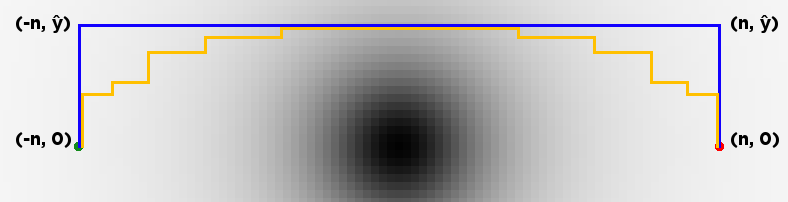
\includegraphics[width=\columnwidth]{graphix/bracket.png}
\caption{The Bracket Shape}
\label{fig:bracket}
\end{figure}

One could easily prove that the optimal path takes such a shape when $f\in\Psi$, by substituting any path that goes closer to the obstacle with one of equal length that goes further away, but we omit such a proof here for space. 


